\documentclass{homework}
\usepackage{bussproofs}
\EnableBpAbbreviations
\usepackage{ctex,hyperref,float,algorithm,algorithmic,pgfplots}

\name{熊泽恩} % Replace (Student Name) with your name.
\id{2022011223}
\term{2024 Spring}
\course{Introduction to Theoretical Computer Science}
\hwnum{10}

%\hwname{(Name)}          % Uncomment and replace (Name) with the type of the
                          % homework (e.g, Assignment, Problem Set, etc.) if you
                          % don't want the document to be labeled as "Homework."
%\problemname{(Name)}     % Uncomment and replace (Name) with the desired label
                          % for problems created with the problem environment.
%\solutionname{(Name)}    % Uncomment and replace (Name) with the desired label
                          % for solutions created with the solution environment.

% Load any other packages you need here.

\begin{document}

\begin{problem}\label{1}
  \begin{parts}
    \part\label{1.a}
    Let $X$ be a random variable taking values in $[0,1]$.
    Prove that if $\E(X) = \eps$, then
    \begin{equation*}
      \Pr \Bigl(X \ge \frac{\eps}{2} \Bigr) \ge \frac{\eps}{2}.
    \end{equation*}
    \part\label{1.b}
    Let $X \ge 0$ be a random variable. Prove that
    \begin{equation*}
      \Pr (X = 0) \le \frac{\Var(X)}{{\bigl(\E(X)\bigr)}^{2}}.
    \end{equation*}
  \end{parts}
\end{problem}

\begin{solution}

  \ref{1.a}

  Let $\mathbf{1}_{x \ge \frac{\eps}{2}}$ be the indicator function of the event $x \ge \frac{\eps}{2}$.
  Then from the figure of the indicator function, we have
  \begin{equation*}
    \mathbf{1}_{x \ge \frac{\eps}{2}} \ge 1 - \frac{\eps}{2x}.
  \end{equation*}

  \begin{center}
    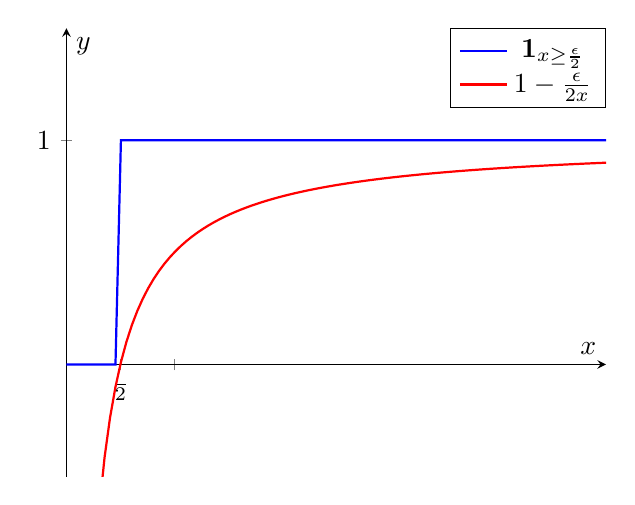
\begin{tikzpicture}
      \begin{axis}[
          domain=0:10,
          samples=100,
          axis lines=middle,
          xlabel={$x$},
          ylabel={$y$},
          ymin=-0.5,
          ymax=1.5,
          xtick={0,1,2},
          ytick={0,1},
          xticklabels={$0$,$\frac{\eps}{2}$},
          yticklabels={$0$,$1$},
          legend style={at={(1,1)},anchor=north east}
      ]
      
      \addplot[blue,thick] {(x>=1)};
      \addlegendentry{$\mathbf{1}_{x \ge \frac{\epsilon}{2}}$}
  
      \addplot[red,thick] {1 - 1/x};
      \addlegendentry{$1 - \frac{\epsilon}{2x}$}
      
      \end{axis}
    \end{tikzpicture}
  \end{center}

  Therefore, we have
  \begin{equation*}
    \Pr \Bigl(X \ge \frac{\eps}{2} \Bigr)
    = \E \bigl( \mathbf{1}_{x \ge \frac{\eps}{2}} \bigr) 
    \ge \E \bigl( 1 - \frac{\eps}{2x} \bigr) = 1 - \frac{\eps}{2\E(x)}
    = \frac{1}{2} \ge \frac{\eps}{2}.
  \end{equation*}

  \ref{1.b}

  From the Chebyshev's inequality, for any $t > 0$, we have
  \begin{equation*}
    \Pr(\abs{X - \E(X)} \ge t) \le \frac{\Var(X)}{t^2}.
  \end{equation*}

  Since $X \in [0, 1]$, then $\E(X) \ge 0$. Let $t = \E(X)$, then
  \begin{align*}
    \Pr(X = 0) & = \Pr(X \le 0) \\
    & \le \Pr(X \le 0 \text{ or } X \ge 2\E(X)) \\
    & = \Pr(\abs{X - \E(X)} \ge \E(X)) \\
    & \le \frac{\Var(X)}{{\bigl(\E(X)\bigr)}^{2}}.
  \end{align*}

\end{solution}

\begin{problem}
  Let $\mathrm{RandomSign}(n)$ be the distribution of vectors of $n$ entries
  where each entry is independently chosen to be $\pm 1$ with probability
  $\frac{1}{2}$.
  Sample $m$ vectors
  $\mathbf{v}^{(1)}, \mathbf{v}^{(2)}, \ldots, \mathbf{v}^{(m)} \sim \mathrm{RandomSign}(n)$.
  Define the normalized vectors $\mathbf{w}^{(i)} = \mathbf{v}^{(i)} / \sqrt{n}$
  so that $\norm{\mathbf{w}^{(i)}} = 1$ for all $i = 1, 2, \ldots, m$.
  Prove the following claims:
  \begin{parts}
    \part\label{2.a} For all $i \ne j$, the inner product
    $\ip{\mathbf{w}^{(i)}}{\mathbf{w}^{(j)}} = \sum_{k} \mathbf{w}^{i}_{k} \mathbf{w}^{j}_{k}$
    is small with high probability.
    That is,
    \begin{equation*}
      \Pr \bigl( \abs{\ip{\mathbf{w}^{(i)}}{\mathbf{w}^{(j)}}} \ge \delta \bigr)
      \le \exp \Bigl( - \Omega \bigl( \delta^{2} n \bigr) \Bigr).
    \end{equation*}
    \part\label{2.b} There exists some $m = \exp (\Omega(\delta^{2} n))$ such that the
    $m$ vectors are pairwise almost-orthogonal with high probability.
    More precisely,
    \begin{equation*}
      \Pr \Bigl( \abs{\ip{\mathbf{w}^{(i)}}{\mathbf{w}^{(j)}}}
      \le \delta \text{ for all pairs } i\ne j \Bigr) \ge 0.99.
    \end{equation*}
    (Note: By probabilistic method, this proves that there are exponentially
    many almost-orthogonal unit vectors in $\real^{n}$ even though there are at most
    $n$ exactly orthogonal vectors.)
  \end{parts}
\end{problem}

\begin{solution}

  \ref{2.a}
  Suppose $\mathbf{w}^{(i)} = (w_1^{(i)}, w_2^{(i)}, \ldots, w_n^{(i)})$
  and $\mathbf{w}^{(j)} = (w_1^{(j)}, w_2^{(j)}, \ldots, w_n^{(j)})$.
  For a fixed $\mathbf{w}^{(j)}$, each entry $w_k^{(j)}$ is chosen
  to be $\frac{1}{\sqrt{n}}$ or $-\frac{1}{\sqrt{n}}$ with equal probability $\frac{1}{2}$.
  Therefore, for any $k \in \{1, 2, \cdots, n\}$, we have $w_k^{(i)} \cdot w_k^{(j)} = \pm \frac{1}{n}$
  with equal probability $\frac{1}{2}$.

  Let $X_k = w_k^{(i)} \cdot w_k^{(j)}$ for $k \in \{1, 2, \cdots, n\}$.
  Then $X_k$ is a random variable taking values in $\left\{ \frac{1}{n}, -\frac{1}{n} \right\}$.
  It is easy to see that $\E(X_k) = 0$ and $\Var(X_k) = \frac{1}{2}\cdot \bigl(1 - \frac{1}{2}\bigr) = \frac{1}{4}$.

  Let $X = \sum_{k} X_k = \sum_{k} w_k^{(i)} \cdot w_k^{(j)} = \abs{\ip{\mathbf{w}^{(i)}}{\mathbf{w}^{(j)}}}$.
  Then $\E(X) = \sum_{k} \E(X_k) = 0$.

  From the Hoeffding's inequality, we have for any $\delta > 0$, if $X_k \in [a_k, b_k]$
  for all $k$, then
  \begin{equation*}
    \Pr \bigl( \abs{X - \E(X)} \ge \delta \bigr)
    \le 2 \exp \Bigl( - \frac{2\delta^2}{\sum_{k} (b_k - a_k)^2} \Bigr).
  \end{equation*}

  Since $\E(X) = 0$, and $X_k \in \left\{ \frac{1}{n}, -\frac{1}{n} \right\}$, then
  \begin{equation*}
    \Pr \bigl( \abs{X} \ge \delta \bigr) \le
    2 \exp \Bigl( - \frac{2\delta^2}{\sum_{k} (\frac{1}{n} - (-\frac{1}{n}))^2} \Bigr).
  \end{equation*}

  That is to say,
  \begin{equation*}
    \Pr \bigl( \abs{\ip{\mathbf{w}^{(i)}}{\mathbf{w}^{(j)}}} \ge \delta \bigr)
    \le 2 \exp \Bigl( - \frac{n\delta^2}{2} \Bigr)
    = \exp \Bigl( - \Omega \bigl( \delta^{2} n \bigr) \Bigr).
  \end{equation*}

  \ref{2.b}
  From \ref{1.a}, we have,
  \begin{equation*}
    \Pr \bigl( \abs{\ip{\mathbf{w}^{(i)}}{\mathbf{w}^{(j)}}} \ge \delta \bigr)
    \le 2 \exp \Bigl( - \frac{n\delta^2}{2} \Bigr), \text{ for all } i \ne j.
  \end{equation*}

  Using the union bound, we have
  \begin{align*}
    & \quad \Pr \Bigl( \abs{\ip{\mathbf{w}^{(i)}}{\mathbf{w}^{(j)}}}
    \le \delta \text{ for all pairs } i\ne j \Bigr) \\
    & \ge 1 - \binom{m}{2} \cdot 2 \exp \Bigl( - \frac{n\delta^2}{2} \Bigr) \\
    & > 1 - m^2 \exp \Bigl( - \frac{n\delta^2}{2} \Bigr) \\
  \end{align*}

  So when $m = \frac{1}{100}\exp \bigl( \frac{n\delta^2}{4} \bigr) = \exp \bigl( \Omega(\delta^2 n) \bigr)$,
  we have
  \begin{equation*}
    \Pr \Bigl( \abs{\ip{\mathbf{w}^{(i)}}{\mathbf{w}^{(j)}}}
    \le \delta \text{ for all pairs } i\ne j \Bigr)
    > 1 - m^2\exp \Bigl( - \frac{n\delta^2}{2} \Bigr)
    = 1-10^{-4} > 0.99.
  \end{equation*}

\end{solution}

\begin{problem}
  Let $\mathrm{RandomGraph}(n, p)$ be the distribution of random graphs of $n$
  vertices where, for each pair of vertices $u, v$, $\{u, v\}$ is chosen as an
  edge of the graph independently with probability $p$.
  Prove the following for such a random graph
  $G \sim \mathrm{RandomGraph}(n,p)$.
  \begin{parts}
    \part\label{3.a} If $p = o(n^{-2/3})$,
    \begin{equation*}
      \lim_{n \to \infty} \Pr(G \text{ contains a $4$-clique}) = 0.
    \end{equation*}
    \part\label{3.b} If $p = \omega(n^{-2/3})$,
    \begin{equation*}
      \lim_{n \to \infty} \Pr(G \text{ does not contain a $4$-clique}) = 0.
    \end{equation*}
    (Hint: Use Part \ref{1.b} of Problem \ref{1} and you need to carefully
    calculate the probability of 4-cliques occurring simultaneously on vertex
    sets $A$ and $B$ when $\abs{A \cap B} \ge 2$.)
  \end{parts}
\end{problem}

\begin{solution}

  Let $X$ be the number of $4$-cliques in the graph. Let $X_S$ be
  the indicator random variable of the event that
  a vertex set $S$ of size $4$ is a $4$-clique.
  Then $X = \sum_{S} X_S$. Since $X_S \in \{0, 1\}$, then $\E(X_S) = p^6$.
  So we have
  \begin{equation*}
    \E(X) = \sum_{S} \E(X_S) = \binom{n}{4} \cdot (p^6 - p^{12}).
  \end{equation*}

  \ref{3.a}
  The probability that there exists a $4$-clique in the graph is
  \begin{equation*}
    \Pr(G \text{ contains a $4$-clique}) = \Pr(X > 0) = \Pr(X \ge 1).
  \end{equation*}

  By Markov's inequality, we have
  \begin{equation*}
    \Pr(X \ge 1) \le \E(X) = \binom{n}{4} \cdot (p^6 - p^{12}) = \Theta(n^4)(p^6-p^{12}).
  \end{equation*}

  Since $p = o(n^{-2/3})$, then $\lim_{n \to \infty}\E(X) = 0$. Therefore,
  \begin{equation*}
    \lim_{n \to \infty} \Pr(G \text{ contains a $4$-clique}) = 0.
  \end{equation*}

  \ref{3.b}
  From Part \ref{1.b} of Problem \ref{1}, we have
  \begin{equation*}
    \Pr(X = 0) \le \frac{\Var(X)}{{\bigl(\E(X)\bigr)}^{2}}.
  \end{equation*}

  Now we need to calculate $\Var(X)$. Rewrite $\Var(X)$ as follows:
  \begin{align*}
    \Var(X) & = \E(X^2) - \E(X)^2 \\
    & = \sum_{S}\E(X_S^2) + \sum_{S \neq T}\E(X_SX_T) - \sum_S \E(X_S)^2 - \sum_{S \neq T}\E(X_S)\E(X_T) \\
    & = \sum_{S}\Var(X_S) + \sum_{S \neq T}\text{Cov}(X_S, X_T).
  \end{align*}

  Since $X_S \in \{0, 1\}$, then $\Var(X_S) = \E(X_S^2) - \E(X_S)^2 = p^6 - p^{12}$.
  So
  \begin{equation*}
    \sum_{S}\Var(X_S) = \binom{n}{4} \cdot (p^6 - p^{12}).
  \end{equation*}

  Now we need to calculate $\text{Cov}(X_S, X_T)$ for $S \neq T$.
  There are 4 cases for $S, T$:
  
  \begin{enumerate}
    \item $S, T$ have $0$ common vertex: It easy to see that $\text{Cov}(X_S, X_T) = 0$.
    \item $S, T$ have $1$ common vertex: Still, $\text{Cov}(X_S, X_T) = 0$.
          This is because there are no common edges between $S$ and $T$.
    \item $S, T$ have $2$ common vertices: In this case, $\E(X_SX_T) = p^{11}$.
          So
          \begin{equation*}
            \text{Cov}(X_S, X_T) = \E(X_SX_T) - \E(X_S)\E(X_T) = p^{11} - p^{12}.
          \end{equation*}
          The number of ways to choose $S, T$ for this case is
          \begin{equation*}
            \binom{n}{6} \cdot \binom{6}{2} \cdot \binom{4}{2} = \Theta(n^6).
          \end{equation*}
    \item $S, T$ have $3$ common vertices: In this case, $\E(X_SX_T) = p^{9}$.
          So
          \begin{equation*}
            \text{Cov}(X_S, X_T) = \E(X_SX_T) - \E(X_S)\E(X_T) = p^{9} - p^{12}.
          \end{equation*}
          The number of ways to choose $S, T$ for this case is
          \begin{equation*}
            \binom{n}{5} \cdot \binom{5}{3} \cdot \binom{2}{1} = \Theta(n^5).
          \end{equation*}
  \end{enumerate}

  By summing up all four cases together, we have
  \begin{align*}
    \text{Cov}(X_S, X_T) & = \Theta(n^6)(p^{11} - p^{12}) + \Theta(n^5)(p^{9} - p^{12}) \\
    & \le \Theta(n^6)p^{11} + \Theta(n^5)p^{9}
  \end{align*}

  So the variance of $X$ is
  \begin{align*}
    \Var(X) & = \sum_{S}\Var(X_S) + \sum_{S \neq T}\text{Cov}(X_S, X_T) \\
    & \le O(n^4p^6) + \Theta(n^6)p^{11} + \Theta(n^5)p^{9}
  \end{align*}

  Therefore, when $p = \omega(n^{-2/3})$,
  \begin{align*}
    & \quad \lim_{n \to \infty} \frac{\Var(X)}{{\bigl(\E(X)\bigr)}^{2}} \\
    & \le \lim_{n \to \infty}\frac{O(n^4p^6) + \Theta(n^6)p^{11} + \Theta(n^5)p^{9}}
    {\Theta(n^4)(p^6 - p^{12})} \\
    & = \lim_{n \to \infty}\frac{O(1) + \Theta(n^2)p^5 + \Theta(n)p^3}{1 - p^6} \\
    & = 0.
  \end{align*}

  Since $\frac{\Var(X)}{{\bigl(\E(X)\bigr)}^{2}} \ge 0$, hence, we have
  \begin{equation*}
    \lim_{n \to \infty} \Pr(G \text{ does not contain a $4$-clique}) = 0.
  \end{equation*}

\end{solution}

\end{document}
